%agestyle{fancy}
%\thispagestyle{plain}
%\pagestyle{fancyplain}
%\lhead[\fancyplain{}{\slshape %\rightmark}]
%\chead{}
%\rhead[\fancyplain{}{\slshape %\leftmark}]
%\lfoot[]{\thepage}
%\cfoot[]{Estadistica I}
%\rfoot{\thepage}
%\setlength{\headrulewidth}{0.4pt}
%\setlength{\footrulewidth}{0.4pt}
%TCIDATA{OutputFilter=latex2.dll}
%TCIDATA{Version=4.00.0.2312}
%TCIDATA{LaTeXparent=0,0,Est12.tex}
%TCIDATA{ChildDefaults=%
%chapter:1,page:1
%}


%\begin{quote}
\bigskip
%\end{quote}

\section{\textquestiondown Qu\'{e} es la estad\'{\i}stica?}

\textit{La estad\'{\i}stica se encarga de establecer los m\'{e}todos y
procedimientos para recolectar, clasificar y resumir datos para luego
analizarlos\ siempre que exista \ variabilidad e incertidumbre causada
intr\'{\i}nsicamente por ellos y despu\'{e}s ralizar inferencias con el fin de
hacer predi\-cciones y tomar decisiones. }

Ahora clasificaremos la estad{\'\i}stica.

\begin{criterion}
Estad\'{\i}stica descriptiva: Describe y analiza los datos utilizando
m\'{e}todos num\'{e}ricos elementales y gr\'{a}ficos para resumir y presentar
la informaci\'{o}n contenida en ellos.
\end{criterion}

\begin{criterion}
Estad\'{\i}stica inferencial: apoy{\'{a}}ndose del c\'{a}lculo de
pro\-ba\-bilidades y utilizando los datos de una muestra, efect\'{u}a
estima\-ciones, decisiones y generaliza sobre un conjunto mayor de datos
llamado poblaci\'{o}n.
\end{criterion}

\section{Organizaci\'{o}n de datos}

Generalmente los datos se organizan usando tablas \ y determinando algunas
cantidades o valores que definiremos a continuaci\'{o}n:

Consideremos una poblaci\'{o}n finita de $n$ elementos o indivi\-duos descrita
seg\'{u}n un car\'{a}cter o variable $X$ cuyas modalidades han sido agrupadas
en un n\'{u}mero $k$ de clases, que denotaremos $\ c_{1},c_{2},c_{3}%
,...,c_{k}$ y para cada clase $c_{i},i=1,2,3,...,k$ definimos lo si\-guiente:
\footnotetext{La poblaci\'{o}n tambi\'{e}n puede ser infinita, pero ese caso
lo estudiaremos m\'{a}s adelante en el cap\'{\i}tulo 3}

\begin{definition}
Frecuencia absoluta: La frecuencia absoluta de una clase $c_{i}$ es el
n\'{u}mero de veces $n_{i}$ que se observa una modalidad perteneciente a esa clase.
\end{definition}

\begin{definition}
Frecuencia relativa: La frecuencia relativa de una clase $c_{i}$ es el
cociente $f_{i}$ entre la frecuencia absoluta de la clase $c_{i}$ y el
n\'{u}mero total de observaciones de todas las modalidades pertenecientes a
todas las clases.
\end{definition}

Generalmente esta frecuencia se multiplica por 100 y se da en porcentaje

\begin{definition}
Frecuencia absoluta acumulada: La frecuencia absoluta acumulada $N_{i}$ es el
n\'{u}mero de elementos de la poblaci\'{o}n cuya modalidad es inferior o
equivalente a la modalidad $c_{i}$ es decir,
\[
N_{i}=\sum_{j=1}^{k}n_{j}%
\]

\end{definition}

\begin{definition}
Frecuencia relativa acumulada: Se denota $F_{i}$ y es el tanto por uno de los
elementos de la poblaci\'{o}n que est\'{a}n en alguna de las clases y que
presenta una modalidad inferior o igual a la $c_{i}$, es decir
\[
F_{i}=\frac{N_{i}}{n}=\sum_{j=1}^{k}f_{j}
\]

\end{definition}

De \'{e}stas definiciones se pueden deducir algunas propiedades evi\-dentes ya
que las modalidades son exhaustivas y mutuamente excluyentes

\begin{itemize}
\item
\[
n=\sum_{j=1}^{k}n_{j}\;,\;\sum_{j=1}^{k}f_{j}%
\]

\end{itemize}



\begin{definition}
Tabla de frecuencia\bigskip: Es una representaci\'{o}n de $\mathfrak{F}$ y
generalmente es de la siguiente forma:%

\begin{tabular}
[c]{||c||c||c||c||c||}\hline\hline
{\small M} & {\small F.} & {\small F.R.} & {\small F.A.A.} & {\small F.R.A.}%
\\\hline\hline
{\small C} & {\small n}$_{i}$ & {\small f}$_{i}$ & {\small N}$_{i}$ &
{\small F}$_{i}$\\\hline\hline
{\small c}$_{1}$ & {\small n}$_{1}$ & {\small f}$_{1}${\small =}$\frac{n_{1}%
}{n}$ & {\small N}$_{1}${\small =n}$_{1}$ & {\small F}$_{1}${\small =}%
$\frac{N_{1}}{n}${\small =f}$_{1}$\\\hline\hline
{\small c}$_{2}$ & {\small n}$_{2}$ & {\small f}$_{2}${\small =}$\frac{n_{2}%
}{n}$ & {\small N}$_{2}${\small =n}$_{1}${\small +n}$_{2}$ & {\small F}$_{2}%
${\small =f}$_{1}${\small +f}$_{2}$\\\hline\hline
{\small c}$_{3}$ & {\small n}$_{3}$ & {\small f}$_{3}${\small =}$\frac{n_{3}%
}{n}$ & {\small N}$_{3}${\small =n}$_{1}${\small +n}$_{2}${\small +n}$_{3}$ &
{\small F}$_{3}${\small =f}$_{1}${\small +f}$_{2}${\small +f}$_{3}%
$\\\hline\hline
$\vdots$ & $\vdots$ & $\vdots$ & $\vdots$ & $\vdots$\\\hline\hline
{\small c}$_{j}$ & {\small n}$_{j}$ & {\small f}$_{j}${\small =}$\frac{n_{j}%
}{n}$ & {\small N}$_{j}${\small =}$\sum_{i=1}^{j}${\small n}$_{i}$ &
{\small F}$_{j}${\small =}$\sum_{i=1}^{j}${\small f}$_{i}$\\\hline\hline
$\vdots$ & $\vdots$ & $\vdots$ & $\vdots$ & $\vdots$\\\hline\hline
{\small c}$_{k}$ & {\small n}$_{k}$ & {\small f}$_{k}${\small =}$\frac{n_{k}%
}{n}$ & {\small N}$_{k}${\small =n} & {\small F}$_{k}${\small =1}%
\\\hline\hline
& {\small n} & {\small 1} &  & \\\hline\hline
\end{tabular}
\footnote{Aunque hemos definido la tabla s\'{o}lo para $\mathfrak{F}$ en
realidad en una tablas de frecuencia se tabulan las otras frecuencias
definidas en este apartado}
\end{definition}

Donde:M: representa modalidades, \newline F.A.:frecuencia absoluta,
F.R.:frecuencia relativa, F.A.A: frecuencia absoluta acumulada y F.R.A.:
frecuencia relativa acumulada.

\begin{example}
Se lanzan cinco monedas 1000 veces. El n\'{u}mero de lanzamientos en los que
han salido 0,1,2,3,4,5 caras se indican en la siguiente tabla:
\[%
\begin{tabular}
[c]{|l|l|l|l|l|}\hline
N%
%TCIMACRO{\U{ba} }%
%BeginExpansion
${{}^o}$
%EndExpansion
de caras & $n_{i}$ & $f_{i}$ & $N_{i}$ & $F_{i}$\\\hline
0 & 38 & $\frac{38}{1000}=\allowbreak\allowbreak0.038\,$ & 38 & 0.038\\\hline
1 & 144 & $\frac{144}{1000}=\allowbreak0.144\,$ & 182 & 0.182\\\hline
2 & 342 & $\frac{342}{1000}=\allowbreak0.342\,$ & 524 & 0.524\\\hline
3 & 287 & $\frac{287}{1000}=\allowbreak0.287\,$ & 811 & 0.811\\\hline
4 & 164 & $\frac{164}{1000}=\allowbreak0.164\,$ & 975 & 0.975\\\hline
5 & 25 & $\frac{25}{1000}=\allowbreak0.025\,$ & 1000 & 1\\\hline
Total & 1000 & 1 &  & \\\hline
\end{tabular}
\
\]
\ \ \ \ \ \ \ \ \ \ \ \ \ \ \ \ \ \ \
\end{example}



\subsubsection{Elecci\'{o}n de clases}

Las clases se pueden seleccionar de diferentes formas, pero siempre hay que
seguir los criterios que se ajustan al tipo de variables que estudiamos.

\begin{itemize}
\item Cuando se trata de una variable nominal las clases $c_{i}$ ser{\'a}n de
tipo nominal

\item Cuando la variable es cuantitativa discreta las clases ser\'{a}n
valo\-res num\'{e}ricos del tipo $x_{1},x_{2},x_{3},\cdots,x_{k}.$

\item Si las variables son cuantitativas continuas las clases se definen
mediante intervalos abiertos o semiabiertos, es decir de la forma:
\[
\left(  x_{i-1},x_{i}\right)  ,\left(  x_{i},x_{i+1}\right)  ,\left[
x_{i-1},x_{i}\right)  ,\left[  x_{i},x_{i+1}\right)  ,\left(  x_{i-1}%
,x_{i}\right]  ,\left(  x_{i},x_{i+1}\right]  .
\]

\end{itemize}

En estos casos las modalidades que contienen una clase son todos los valores
num\'{e}ricos posibles contenidos en el intervalo.

Por convenci\'{o}n nosotros de qu\'{\i} en adelante tomaremos siempre los
$(k-1)$ primeros intervalos de la forma $\left(  x_{i-1},x_{i}\right]  $ y el
\'{u}ltimo $[x_{k-1},x_{k}].$ A cada intervalo lo representaremos
$x_{i-1}-x_{i}=I_{i}$.

\begin{definition}
Amplitud: La amplitud de un intervalo se define $a_{i}=x_{i}-x_{i-1}.$
\end{definition}

\begin{definition}
Marca de clase: Es un valor $m_{i}$ $\in I_{i\text{ }}$que representa a la
clase y se define
\[
m_{i}=\frac{x_{i}+x_{i-1}}{2}
\]

\end{definition}

La marca de clase es una forma abreviada de representar la clase.

Nota: $m_{i}$ se determina de esta forma si las clases son conjuntos acotados.

\subsubsection{Elecci\'{o}n de clases para variables continuas}

Cuando tenemos una muestra es importante escoger en una forma adecuada las
clases y el num\'{e}ro de clases $k$ y para ello indicaremos los siguientes pasos:

\begin{itemize}
\item Lo primero es determinar $k$, entre mayor sea su valor mejor\footnote{Se
aconseja que se escojan entre 5 y 20 clases dependiendo del n\'{u}mero de
datos}, pero de todas formas hay que acotarlo por que la idea es reducir el
n\'{u}mero de datos en la muestra.
\[
k=\left\{
\begin{array}
[c]{cc}%
\sqrt{n} & \text{si }n\text{ es muy grande}\\
1+3.22\log n & \text{en otro caso}%
\end{array}
\right\}
\]

\end{itemize}

$n$ se considera grande si $n\geq40$

\begin{itemize}
\item Como segundo paso se determina el rango $R=x_{k}-x_{0}$

\item Determinado el rango de la muestra podemos hallar la amplitud de cada
intervalo que generalmente la tomamos constante:
\[
a=\frac{R}{k},\quad a_{i}=a\quad\forall i=1,2,3,...,k
\]


\item Ahora determinaremos los intervalos\footnote{Se aconseja que las marcas
de clases coincidan con un gran n\'{u}mero de datos y que los datos no sean
extremos de las clases, para que los c{\'a}lculos posteriores queden mejor
aproximados.}
\end{itemize}

%

\begin{align*}
x_{0}  &  =x_{\min}\\
x_{1}  &  =x_{0}+a\\
x_{2}  &  =x_{1}+2a\\
x_{k}  &  =x_{\max}+ka
\end{align*}


Como se puede observar es posible que el valor de $a$ no sea un n\'{u}mero
f\'{a}cil de manejar entonces en estos casos como
\[
x_{k}\geq x_{\max}>x_{\min}\geq x_{0}
\]
entonces se var\'{\i}an los extremos sim{\'e}tricamente y $a$ se aproxima al
mayor entero es decir $a\prime=\left[  \left[  a\right]  \right]  +1$

\begin{example}
Queremos observar el peso de las personas en una poblaci\'{o}n y se toma una
muestra de 21 individuos, los cuales est{\'a}n tabulados en la siguiente tabla
\end{example}

$
\begin{tabular}
[c]{l}%
Peso en Kg\\%
\begin{tabular}
[c]{lllllll}%
58 & 42 & 51 & 54 & 40 & 40 & 49\\
56 & 58 & 57 & 59 & 63 & 58 & 66\\
70 & 73 & 71 & 69 & 70 & 68 & 64
\end{tabular}
\end{tabular}
$

Determinar una tabla de frecuencias:

\begin{solution}
Lo primero que hay que identificar es la variable y en este caso vemos que la
variable es de tipo cuantitativa continua por lo que ahora hay que determinar
los intervalos y su longitud para que la perdida de informaci\'{o}n no sea
significativa entonces sea $X$ la variable peso, utilizaremos la f\'{o}mula
$k=1+3.22\ast\log_{10}21=5.\,\allowbreak257\,5\approxeq6$ aunque podr{\'\i
}amos escoger tambi\'{e}n $k=\sqrt{21}\approxeq5$.
\end{solution}

Ahora hallemos $R=73-40=33\Longrightarrow a_{i}=a=\frac{33}{6}=5.\,\allowbreak
5$

$x_{0}=x_{\min}=40$

$x_{5}=x_{\max}=73$%
\[%
\begin{tabular}
[c]{||c||c||c||c||c||c||c||}\hline\hline
$i$ & Intervalos & $m_{i}$ & $n_{i}$ & $f_{i}$ & $N_{i}$ & $F_{i}%
$\\\hline\hline
1 & 40-45,5 &  &  &  &  & \\\hline\hline
2 & 45,5-51 &  &  &  &  & \\\hline\hline
3 & 51-56,5 &  &  &  &  & \\\hline\hline
4 & 56,5-62 &  &  &  &  & \\\hline\hline
5 & 62-67.5 &  &  &  &  & $\thickapprox1$\\\hline\hline
6 & 67,5-73 &  &  &  & 21 & $\thickapprox1$\\\hline\hline
Total &  &  & 21 & $\thickapprox1$ &  & \\\hline\hline
\end{tabular}
\
\]




Utilizando un software estad\'{\i}stico obtenemos la siguiente tabla%
%TCIMACRO{\FRAME{dhF}{11.1017cm}{6.6009cm}{0pt}{}{}{peso.wmf}%
%{\special{ language "Scientific Word";  type "GRAPHIC";
%maintain-aspect-ratio TRUE;  display "USEDEF";  valid_file "F";
%width 11.1017cm;  height 6.6009cm;  depth 0pt;  original-width 8.6948in;
%original-height 5.1526in;  cropleft "0";  croptop "0.9977";
%cropright "0.9989";  cropbottom "0";
%filename '../Tacho/peso.WMF';file-properties "XNPEU";}}}%
%BeginExpansion
\begin{center}
\includegraphics[
trim=0.000000in 0.000000in 0.009564in 0.011851in,
natheight=5.152600in,
natwidth=8.694800in,
height=6.6009cm,
width=11.1017cm
]%
{peso.png}%
\end{center}
%EndExpansion


\section{Representaciones gr\'{a}ficas y diagramas}

En la secci\'{o}n anterior hemos visto que al organizar los datos en una tabla
se reduce la informaci\'{o}n, pero con ello podemos analizarlos de manera
m\'{a}s sistem\'{a}tica y de esa manera podemos concentrarnos en los m\'{a}s
importante, pero a\'{u}n as\'{\i} a veces no es f\'{a}cil observar todo lo que
queremos, sobre todo si la persona interesada en los resultados no le interesa
la estad\'{\i}stica y sabe muy poco de ella, por lo que una representaci\'{o}n
gr\'{a}fica simplifica a\'{u}n m\'{a}s los datos.

\subsection{Gr\'{a}ficos para variables cualitativas}

\begin{description}
\item[i.] Diagramas de barras

Se establece una especie de plano cartesiano representando las modalidades en
el eje de ordenadas y las frecuencias absolutas o relativas en el eje de las
abscisas, con este gr\'{a}fico \ si\ se comparan varias poblaciones entre
s\'{\i} es conveniente utilizar las frecuencias relativas
\end{description}

%\begin{quote}%
%TCIMACRO{\FRAME{dhFU}{9.3818cm}{4.8436cm}{0pt}{\Qcb{Diagrama de barra para una
%variable cualitativa}}{\Qlb{ec1}}{estadoc.wmf}%
%{\special{ language "Scientific Word";  type "GRAPHIC";
%maintain-aspect-ratio TRUE;  display "USEDEF";  valid_file "F";
%width 9.3818cm;  height 4.8436cm;  depth 0pt;  original-width 7.6527in;
%original-height 3.9306in;  cropleft "0";  croptop "0.9977";
%cropright "0.9996";  cropbottom "0";
%filename '../Tacho/estadoc.WMF';file-properties "XNPEU";}}}%
%BeginExpansion
\begin{center}
\includegraphics[
trim=0.000000in 0.000000in 0.003061in 0.009040in,
natheight=3.930600in,
natwidth=7.652700in,
height=4.8436cm,
width=9.3818cm
]%
{estadoc.png}%
\\
Diagrama de barra para una variable cualitativa
\label{ec1}%
\end{center}
%EndExpansion%
%TCIMACRO{\FRAME{fphFU}{8.5668cm}{9.4784cm}{0pt}{\Qcb{AREAS DE LOS
%CONTINENTES}}{}{areac.wmf}{\special{ language "Scientific Word";
%type "GRAPHIC";  maintain-aspect-ratio TRUE;  display "USEDEF";
%valid_file "F";  width 8.5668cm;  height 9.4784cm;  depth 0pt;
%original-width 9.5553in;  original-height 10.5836in;  cropleft "0";
%croptop "1";  cropright "1";  cropbottom "0";
%filename '../Tacho/Areac.wmf';file-properties "XNPEU";}}}%
%BeginExpansion
\begin{center}
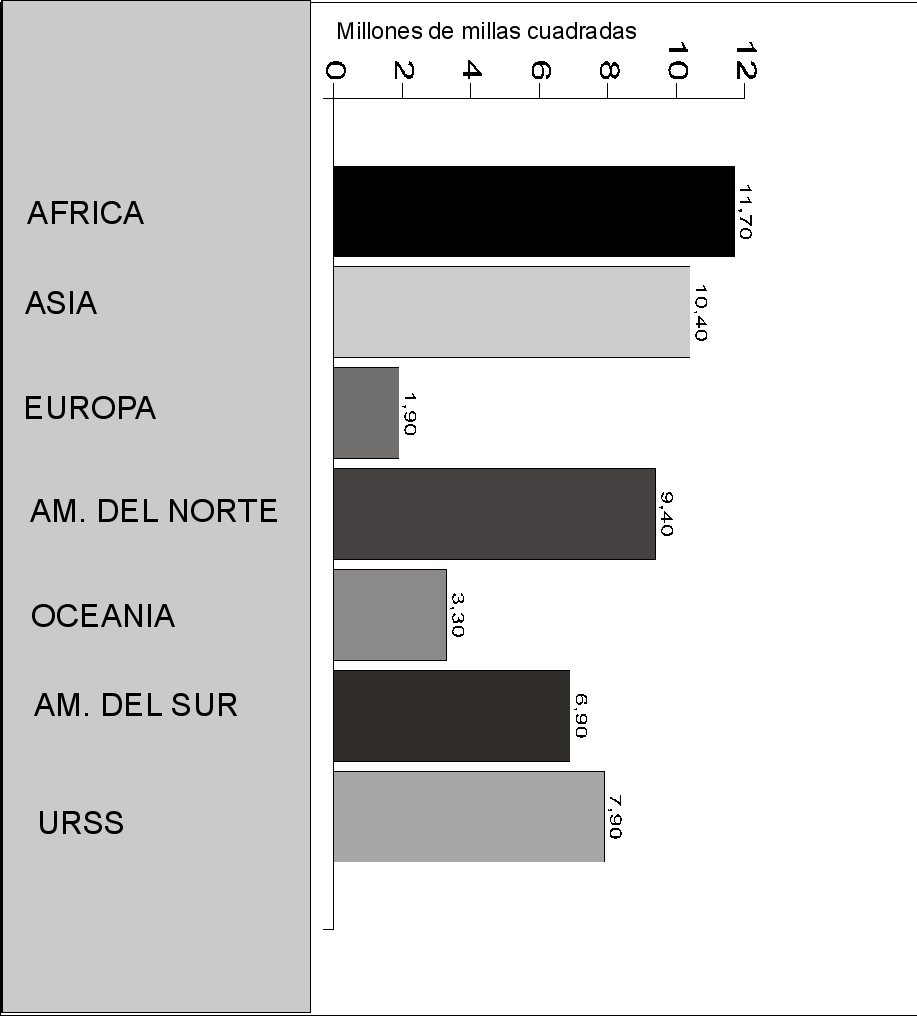
\includegraphics[width=3cm]{Areac.png}
\end{center}

AREAS DE LOS CONTINENTES
\label{ec1}%
\bigskip

\begin{description}
\item \bigskip\lbrack ii.] Diagramas circulares o sectores:
\end{description}

En estos diagramas se toma un c\'{\i}rculo o cilindro y se dividen en tantos
sectores como clases existan de modo que cada sector es proporcional a su
frecuencia absoluta o acumulada, como se indica en los siguientes diagramas:%
%TCIMACRO{\FRAME{dtbpFU}{8.2549cm}{10.3175cm}{0pt}{\Qcb{Diagrama circular}}%
%{}{feconomia.wmf}{\special{ language "Scientific Word";  type "GRAPHIC";
%maintain-aspect-ratio TRUE;  display "USEDEF";  valid_file "F";
%width 8.2549cm;  height 10.3175cm;  depth 0pt;  original-width 8.0557in;
%original-height 10.6804in;  cropleft "0";  croptop "1";  cropright "1";
%cropbottom "0";  filename '../Tacho/feconomia.WMF';file-properties "XNPEU";}%
%}}%
%BeginExpansion
\begin{center}
\includegraphics[
natheight=10.680400in,
natwidth=8.055700in,
height=10.3175cm,
width=8.2549cm
]%
{feconomia.png}%
\\
Diagrama circular
\end{center}
%EndExpansion
\subsection{Gr\'{a}ficos para variables cuantitativas}

\begin{description}
\item[i.] Diagrama de puntos: En este diagrama se coloca la frecuencia
absoluta o relativa de una modalidad en una recta num\'{e}rica y nos sirve
para analizar dos o m\'{a}s modalidades cuando el n\'{u}mero de datos es
peque\~{n}o, con este gr\'{a}fico analizamos f\'{a}cilmente la tendencia y la
variabilidad de la muestra. lo mismo que caracter\'{\i}sticas poco usuales.%
%TCIMACRO{\FRAME{dtbpF}{3.7446in}{1.1978in}{0pt}{}{}{punto.eps}%
%{\special{ language "Scientific Word";  type "GRAPHIC";
%maintain-aspect-ratio TRUE;  display "USEDEF";  valid_file "F";
%width 3.7446in;  height 1.1978in;  depth 0pt;  original-width 4.3734in;
%original-height 1.6968in;  cropleft "0";  croptop "1";  cropright "1";
%cropbottom "0";  filename '../Tacho/punto.EPS';file-properties "XNPEU";}}}%
%BeginExpansion
\begin{center}
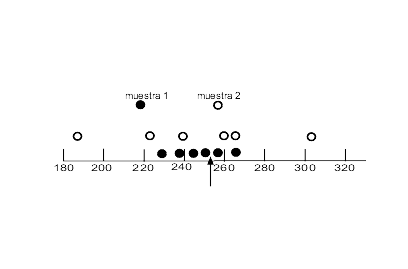
\includegraphics[width=10cm]{punto.png}
\end{center}

%EndExpansion
\item[ii.] Diagrama de tallo y hoja: Cuando el conjunto de datos
\[
x_{1},x_{2},x_{3},\cdots,x_{n}.x_{1},x_{2},x_{3},\cdots,x_{n}.
\]
es grande cada $x_{i},\quad i=1,2,3,...,n$ tiene m\'{a}s de dos d\'{\i}gitos,
entonces se dividen los $x_{i}$ en dos partes
\end{description}

\bigskip Un tallo formado por los primeros d\'{\i}gitos

\bigskip Una hoja formada por el resto de d\'{\i}gitos

\begin{example}
\bigskip En un examen de clasificaci\'{o}n para seleccionar alumnos que pueden
ver directamente c\'{a}lculo en el primer semestre en la facultad de
ingenier\'{\i}a se obtuvieron los siguientes resultados:
\end{example}

\bigskip\ $\left[
\begin{array}
[c]{cccccccccc}%
95 & 95 & 100 & 100 & 100 & 100 & 100 & 105 & 105 & 105\\
110 & 110 & 110 & 110 & 110 & 110 & 110 & 110 & 110 & 115\\
115 & 115 & 115 & 115 & 115 & 115 & 115 & 115 & 115 & 115\\
120 & 120 & 120 & 120 & 120 & 120 & 120 & 120 & 125 & 125\\
125 & 125 & 130 & 130 & 130 & 130 & 135 & 135 & 140 & 140
\end{array}
\right]  \allowbreak$

$\text{%
\begin{tabular}
[c]{l||llllllllllllllllllll}%
{\tiny 09} & {\tiny 5} & {\tiny 5} & {\tiny -} & {\tiny -} & {\tiny -} &
{\tiny -} & {\tiny -} & {\tiny -} & {\tiny -} & {\tiny -} & {\tiny -} &
{\tiny -} & {\tiny -} & {\tiny -} & {\tiny -} & {\tiny -} & {\tiny -} &
{\tiny -} & {\tiny -} & {\tiny -}\\
{\tiny 10} & {\tiny 0} & {\tiny 0} & {\tiny 0} & {\tiny 0} & {\tiny 0} &
{\tiny 5} & {\tiny 5} & {\tiny 5} & {\tiny -} & {\tiny -} & {\tiny -} &
{\tiny -} & {\tiny -} & {\tiny -} & {\tiny -} & {\tiny -} & {\tiny -} &
{\tiny -} & {\tiny -} & {\tiny -}\\
{\tiny 11} & {\tiny 0} & {\tiny 0} & {\tiny 0} & {\tiny 0} & {\tiny 0} &
{\tiny 0} & {\tiny 0} & {\tiny 0} & {\tiny 0} & {\tiny 5} & {\tiny 5} &
{\tiny 5} & {\tiny 5} & {\tiny 5} & {\tiny 5} & {\tiny 5} & {\tiny 5} &
{\tiny 5} & {\tiny 5} & {\tiny 5}\\
{\tiny 12} & {\tiny 0} & {\tiny 0} & {\tiny 0} & {\tiny 0} & {\tiny 0} &
{\tiny 0} & {\tiny 0} & {\tiny 0} & {\tiny 5} & {\tiny 5} & {\tiny 5} &
{\tiny 5} & {\tiny -} & {\tiny -} & {\tiny -} & {\tiny -} & {\tiny -} &
{\tiny -} & {\tiny -} & {\tiny -}\\
{\tiny 13} & {\tiny 0} & {\tiny 0} & {\tiny 0} & {\tiny 0} & {\tiny 5} &
{\tiny 5} & {\tiny -} & {\tiny -} & {\tiny -} & {\tiny -} & {\tiny -} &
{\tiny -} & {\tiny -} & {\tiny -} & {\tiny -} & {\tiny -} & {\tiny -} &
{\tiny -} & {\tiny -} & {\tiny -}\\
{\tiny 14} & {\tiny 0} & {\tiny 0} & {\tiny -} & {\tiny -} & {\tiny -} &
{\tiny -} & {\tiny -} & {\tiny -} & {\tiny -} & {\tiny -} & {\tiny -} &
{\tiny -} & {\tiny -} & {\tiny -} & {\tiny -} & {\tiny -} & {\tiny -} &
{\tiny -} & {\tiny -} & {\tiny -}%
\end{tabular}
}$

{\tiny \bigskip}

\begin{description}
\item[iii.] Diagramas diferenciales: Son aquellos en los que se representan
gr\'{a}ficamente frecuencias absolutas y relativas

\item[iv.] Diagramas integrales: Son los diagramas en los que se representan
gr\'{a}ficamente el n\'{u}mero de elementos que presentan una modalidad
inferior o igual a una modalidad dada y se generan a tr\'{a}ves de las
frecuencias acumuladas
\end{description}

Debido a que existen dos tipos de variables cuantitativas entonces debemos
clasificar estos dos tipos de diagramas de acuerdo con el tipo de variable
cuantitativa en estudio.

\paragraph{Gr\'{a}ficos para variables discreta}

Al representar gr\'{a}ficamente la frecuencia absoluta o relativa de una
variable discreta usamos los diagrama de barras, pero a diferencia de los
diagrama de barra de las variables cualitativas las barras aqu\'{\i} se
presentan con l{\'\i}neas delgadas, para indicar as\'{\i} la naturaleza de la
variable. En el caso de los diagramas integrales tienen la forma del
gr\'{a}fico de una funci\'{o}n escalonada

\begin{example}
La siguiente tabla representa el num\'{e}ro de hijos que ten\'{\i}an 12
familias encuestadas de un caser\'{\i}o cerca a Baranoa:
\[%
\begin{tabular}
[c]{||l||l||l||l||}\hline\hline
$x_{i}$ & $n_{i}$ & $f_{i}$ & $N_{i}$\\\hline\hline
1 & 1 &  & \\\hline\hline
2 & 3 &  & \\\hline\hline
3 & 5 &  & \\\hline\hline
4 & 3 &  & \\\hline\hline
& 12 &  & \\\hline\hline
\end{tabular}
\
\]%
%TCIMACRO{\FRAME{fhFU}{9.5333cm}{5.0676cm}{0pt}{\Qcb{FRECUENCIAS ABSOLUTAS}}%
%{}{barah.wmf}{\special{ language "Scientific Word";  type "GRAPHIC";
%maintain-aspect-ratio TRUE;  display "USEDEF";  valid_file "F";
%width 9.5333cm;  height 5.0676cm;  depth 0pt;  original-width 6.9444in;
%original-height 3.6668in;  cropleft "0";  croptop "1";  cropright "1";
%cropbottom "0";  filename '../Tacho/barah.WMF';file-properties "XNPEU";}} }%
%BeginExpansion
\begin{center}
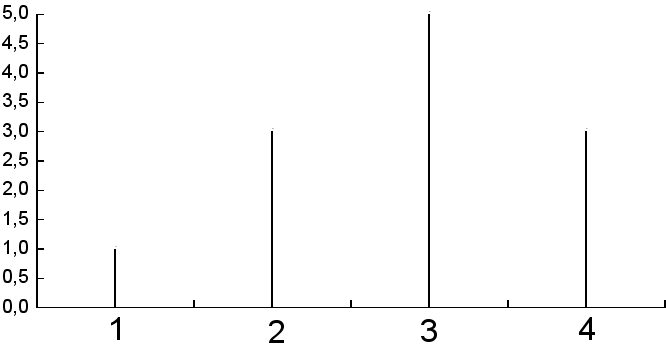
\includegraphics[width=8cm]{barah.png}
\end{center}
\begin{center}{FRECUENCIAS ABSOLUTAS}
\end{center}
%%EndExpansion
%%TCIMACRO{\FRAME{dtbpFU}{7.8024cm}{6.1505cm}{0pt}{\Qcb{FRECUENCIAS ABSOLUTAS
%%ACUMULADAS}}{}{barah1.wmf}{\special{ language "Scientific Word";
%%type "GRAPHIC";  maintain-aspect-ratio TRUE;  display "USEDEF";
%%valid_file "F";  width 7.8024cm;  height 6.1505cm;  depth 0pt;
%%original-width 7.5974in;  original-height 5.9586in;  cropleft "0";
%%croptop "1";  cropright "1";  cropbottom "0";
%%filename '../Tacho/barah1.WMF';file-properties "XNPEU";}} }%
%%BeginExpansion
%\begin{center}
%\includegraphics[
%natheight=5.958600in,
%natwidth=7.597400in,
%height=6.1505cm,
%width=7.8024cm
%]%
%{barah1.png}%
%\end{center}
%\begin{center}{FRECUENCIAS RELATIVAS}
%\end{center}
%%EndExpansion
%Para las variables continuas tambi\'{e}n se pueden representar con diagramas circulares
%\end{example}
%
%\begin{example}
%La tabla representa las notas obtenidas por los alumnos de \ 11%
%%TCIMACRO{\U{ba} }%
%%BeginExpansion
%${{}^o}$
%%EndExpansion
%en un examen de Matem\'{a}ticas en 1990
%\begin{equation}%
%\begin{tabular}
%[c]{ccc}\hline
%\textbf{Notas} & \textbf{Frecuencia} & \textbf{\ frecuencia Relativa}\\\hline
%$10\ $ & $2$ & $2/15=.133$\\
%$9$ & $3$ & $3/15=.200$\\
%$8$ & $4$ & $4/15=.267$\\
%$7$ & $4$ & $4/15=.267$\\
%$4$ & $2$ & $2/15=.133$%
%\end{tabular}
%\ \tag{Tabla 1}%
%\end{equation}%
%\begin{equation}%
%\begin{tabular}
%[c]{cccccccccc}\hline
%\textbf{notas} & $\mathbf{n}_{i}$ &  & \textbf{f}$_{i}$ &  & $f_{i}$
%\textbf{\%} &  & $\mathbf{N}_{i}$ &  & $\mathbf{F}_{i}$\\\hline
%$10\ $ & $2$ &  & $2/15=.133$ &  & $13.3$ &  & $15$ &  & $1.000$\\
%$9$ & $3$ &  & $3/15=.200$ &  & $20.0$ &  & $13$ &  & $.867$\\
%$8$ & $4$ &  & $4/15=.267$ &  & $26.7$ &  & $10$ &  & $.667$\\
%$7$ & $4$ &  & $4/15=.267$ &  & $26.7$ &  & $6$ &  & $.400$\\
%$4$ & $2$ &  & $2/15=.133$ &  & $13.3$ &  & $2$ &  & $.133$%
%\end{tabular}
%\ \tag{Tabla 2}%
%\end{equation}
%%
%\end{example}
%
%\paragraph{Gr\'{a}ficos para variables continuas}
%
%Para las variables continuas existen dos tipos de gr\'{a}ficos:
%
%\begin{itemize}
%\item Los histogramas: Los cuales se construyen representando sobre cada
%intervalo, un rect\'{a}ngulo que tiene la longitud del segmento como base y la
%altura debe ser un valor proporcional a el valor de la frecuencia para ese intervalo.
%
%\item Pol{\'\i}gono de frecuencias: Este se elabora uniendo los puntos que
%corresponden a las im{\'a}genes de las marcas de clase.
%\end{itemize}
%
%En el caso de los diagramas integrales a estos pol{\'\i}gonos se les llama
%ojiva y se obtienen uniendo las abscisas a partir de los extremos de los
%intervalos en los que se han organizado los datos
%
%\begin{example}
%Representar gr\'{a}ficamente la informaci\'{o}n que apare\-ce en la siguiente tabla
%\end{example}
%
%%
%
%\begin{tabular}
%[c]{||c||c||c||c||}\hline\hline
%Intervalos & $m_{i}$ & $n_{i}$ & $N_{i}$\\\hline\hline
%0-2 & 1 & 1 & \\\hline\hline
%2-4 & 3 & 4 & \\\hline\hline
%4-6 & 5 & 10 & \\\hline\hline
%6-8 & 7 & 3 & \\\hline\hline
%8-10 & 9 & 1 & \\\hline\hline
%&  &  & \\\hline\hline
%\end{tabular}
%%TCIMACRO{\FRAME{dhFU}{6.7173cm}{5.0676cm}{0pt}{\Qcb{Diagrama Diferencial}}%
%%{}{hisc.wmf}{\special{ language "Scientific Word";  type "GRAPHIC";
%%maintain-aspect-ratio TRUE;  display "USEDEF";  valid_file "F";
%%width 6.7173cm;  height 5.0676cm;  depth 0pt;  original-width 7.2082in;
%%original-height 5.4163in;  cropleft "0";  croptop "1";  cropright "1";
%%cropbottom "0";  filename '../Tacho/hisc.WMF';file-properties "XNPEU";}} }%
%%BeginExpansion
%\begin{center}
%\includegraphics[
%natheight=5.416300in,
%natwidth=7.208200in,
%height=5.0676cm,
%width=6.7173cm
%]%
%{hisc.png%
%\end{center}
%Diagrama Diferencial
%%EndExpansion
%%TCIMACRO{\FRAME{dhFU}{7.3916cm}{5.4191cm}{0pt}{\Qcb{Pol\'{\i}gono de
%%frecuencias}}{}{poligono.wmf}{\special{ language "Scientific Word";
%%type "GRAPHIC";  maintain-aspect-ratio TRUE;  display "USEDEF";
%%valid_file "F";  width 7.3916cm;  height 5.4191cm;  depth 0pt;
%%original-width 6.8614in;  original-height 5.0142in;  cropleft "0";
%%croptop "1";  cropright "1";  cropbottom "0";
%%filename '../Tacho/poligono.WMF';file-properties "XNPEU";}} }%
%%BeginExpansion
%\begin{center}
%\includegraphics[
%natheight=5.014200in,
%natwidth=6.861400in,
%height=5.4191cm,
%width=7.3916cm
%]%
%{poligono.png}
%\end{center}
%Pol\'{\i}gono de frecuencias
%%EndExpansion
%%TCIMACRO{\FRAME{dhFU}{7.9298cm}{5.3773cm}{0pt}{\Qcb{Diagrama acumulado}}%
%%{}{acumu.wmf}{\special{ language "Scientific Word";  type "GRAPHIC";
%%maintain-aspect-ratio TRUE;  display "USEDEF";  valid_file "F";
%%width 7.9298cm;  height 5.3773cm;  depth 0pt;  original-width 7.7357in;
%%original-height 5.2226in;  cropleft "0";  croptop "1";  cropright "1";
%%cropbottom "0";  filename '../Tacho/Acumu.wmf';file-properties "XNPEU";}} }%
%%BeginExpansion
%\begin{center}
%\includegraphics[width=8cm]{Acumu.png}
%\end{center}
%\begin{center}
%Diagrama acumulado
%\end{center}
%EndExpansion
